% ----------------------------------------------------------
\chapter{A Mecânica do contínuo} \label{Cap:MecCont}
% ----------------------------------------------------------

\section{Cinemática}
A cinemática é responsável pela descrição do movimento, mas desconsidera as forças envolvidas para gera-lo. A mecânica clássica descreve corpos como pontos no espaço. Sua descrição é limitada às quantidades cinemáticas deste único ponto, que normalmente é o centro de massa. De acordo com \cite{gurtin_fried_anand_2013} a propriedade básica de um corpo na mecânica do contínuo é que ele pode ocupar uma região do espaço euclideano. Além disso, de acordo com \cite{tadmor_miller_elliott_2012}, a descrição do corpo não considera a estrutura que o constitui. Em um material descrito pela mecânica do contínuo importam apenas as propriedades verificadas em estado macroscópico. Neste viés, o seccionamento de qualquer corpo A, gerando os corpos B e C, faria com que as propriedades de B e C fossem iguais às de A.  \par

Para \cite{hiermaier_2008} o corpo pode ser descrito como um acúmulo contínuo de pontos no espaço. Dois pontos não podem ocupar o mesmo espaço e um ponto não pode ocupar mais de uma posição ao mesmo tempo. O sistema de coordenadas mais utilizado na mecânica do contínuo é o retangular cartesiano. No qual \ref{eq:kron} e\ref{eq:levi} são válidos. 
\begin{equation} \label{eq:kron}
    \boldsymbol{e_i \cdot e_j} = \gls{deltaK} = \left \{ \begin{array}{rcl}
       0  & \mbox{se} & i \neq j  \\
       1  & \mbox{se} & i = j
    \end{array} \right.
\end{equation}

Onde $ \gls{deltaK} $ é o símbolo de Kronecker Delta.

\begin{equation} \label{eq:levi}
    \boldsymbol{e_i \times e_j} = \gls{levicivita}\boldsymbol{e_k}
\end{equation}

Onde $ \gls{levicivita} $ é o Símbolo de Levi Civita. No qual 
\begin{equation}
    \gls{levicivita} = \left \{ \begin{array}{rcl}
       1  & \mbox{Para permutações pares de ijk.} & \mbox{ex: } 123  \\
       -1  & \mbox{Para permutações impares de ijk.} & \mbox{ex: } 132  \\
       0  & \mbox{se houver repetição nos índices.} 
    \end{array} \right.
\end{equation}

A mecânica do contínuo usa dois espaços para descrever o corpo. O primeiro é fictício e nele estão definidos os nomes das partículas do corpo. Já que o corpo pode ser descrito por um acúmulo contínuo de pontos, então nomear as partículas do corpo usando pontos no espaço é conveniente, portanto o nome de cada partícula do corpo neste espaço é simplesmente sua posição. Por conta de ser usado para nomear as partículas o primeiro espaço é chamado de espaço de referência. O segundo é real no sentido de que neste espaço o corpo pode ser observado e medido, tal que \cite{gurtin_fried_anand_2013} chama este de espaço observado. No espaço de referência reside a configuração do corpo chamada de material. Coordenadas referentes à configuração de referência e portanto do seu correspondente espaço serão denotadas com letras maiúsculas ou com um subíndice $r$. Estas as notações normalmente usadas para diferenciar coordenadas da configuração material. Espacial ou deformada é a configuração do corpo no espaço chamado aqui de real ou observado. Coordenadas referentes à configuração espacial serão denotadas com letra minúscula. Tensores serão sempre denotados por letras maiúsculas e negritadas, não importando a configuração a qual pertencem. \\

Usando estas configurações existem duas descrições mais utilizadas, vide figura \ref{fig:Euler_Lagrange}:
\begin{itemize}
    \item Descrição lagrangiana, material ou referencial: As variáveis independentes são $ \boldsymbol{X} $ e $ t$. O foco aqui é na partícula viajando no tempo. Sendo esta descrição a preferencial quando se fala em mecânica dos sólidos.
    \item Euleriana ou espacial: As variáveis independentes são $ \boldsymbol{x} $ e $ t $. Nesta o foco está em uma posição do espaço, não importando qual partícula a assume em um determinado instante de tempo. Sendo esta a descrição preferencial na mecânica dos fluídos.
\end{itemize}

\begin{figure}[H]
    \centering
    \caption{Representação das diferentes descrições de um corpo.}
    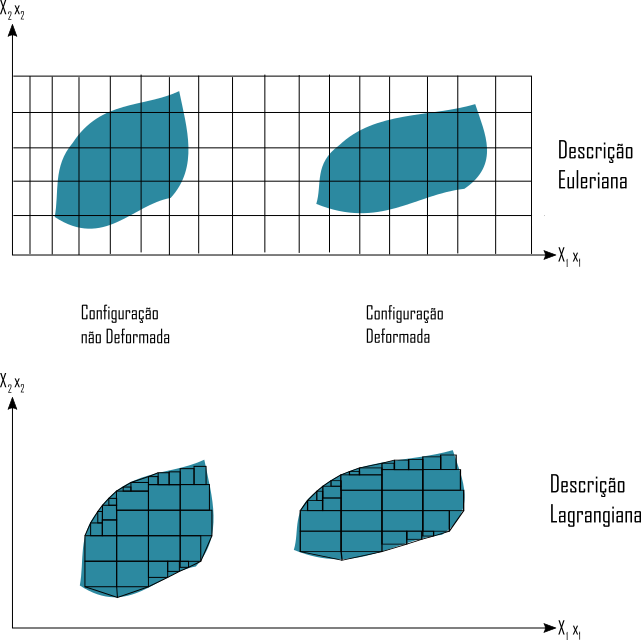
\includegraphics[width=0.8\linewidth]{images/EulervsLagrange.png}
    \label{fig:Euler_Lagrange}
    \fonte{O autor(2020)}
\end{figure}

%Figuras como a \ref{fig:Euler_Lagrange} podem ser vistas como inadequadas por especialistas na mecãnica do contínuo, já que representam no mesmo sistema as coordenadas de referência e espaciais. É necessário explicitar que os dois, embora sejam espaços euclideanos, são diferentes. A representação na figura se vale de um caso particular muito comum em que a configuração de referência e a espacial estão descritas com os mesmos vetores de base e são coincidentes em $ t=0 $. Além disso a figura \ref{fig:Euler_Lagrange} apela para a existência de uma malha, inserida no contexto do método dos elementos finitos, para representar a diferença entre as descrições, porém o método os elementos finitos nada mais é do que uma ferramenta para resolver as equações de equilíbrio. As descrições Lagrangianas e Eulerianas são indepentes do método de solução. \par

Dado que um corpo contínuo pode ser chamado de uma aglomeração de pontos no espaço, então o movimento de uma partícula pode ser representado pelo vetor deslocamento. Que em sua descrição lagrangiana corresponde à expressão \ref{eq:desl_lag}, em sua descrição euleriana corresponde à \ref{eq:desl_euler}.
\begin{align}
&\boldsymbol{U}(\boldsymbol{X},t) = \mathcal{X}(\boldsymbol{X},t) - \boldsymbol{X}
\label{eq:desl_lag}\\
&\boldsymbol{u}(\boldsymbol{x},t) = \boldsymbol{x} - \mathcal{X}^{-1}(\boldsymbol{x},t)
\label{eq:desl_euler}
\end{align}

Onde a função de movimento $ \mathcal{X} $ é tal que $ \boldsymbol{x} = \mathcal{X}(\boldsymbol{X},t) $. Observa-se que , como é de se esperar, $ \boldsymbol{u}(\boldsymbol{x},t) =  \boldsymbol{U}(\boldsymbol{X},t)  $, já que ambos representam o campo de deslocamentos descrito de formas diferentes. \par

A descrição dos deslocamentos torna possível descrever também as deformações.\footnote{É importante notar que há um acumulo de termos quando se trata da mecânica do contínuo em português. O atual assunto é traduzido como deformação, porém em inglês trata-se de "deformation". O conceito da deformação usual, que é causadora de tensões, será abordado nas próximas seções, porém este em inglês chama-se "strain". Por hora a diferença não é pronunciada, porém no futuro ela será novamente citada.} O campo primordial quando se descreve deformações é o gradiente da deformação $ \boldsymbol{F} $, eq. \ref{eq:desl_grad}.

\begin{align}\label{eq:desl_grad}
    \boldsymbol{F}(\boldsymbol{X},t) = \boldsymbol{F} \\
    F_{ij} = \frac{\partial \mathcal{X}_i}{\partial X_j}
\end{align}

Existem deformações homogêneas e não homogêneas. Basicamente as deformações homogêneas são aquelas onde o gradiente da deformação é independe da posição no corpo. De forma geral pode se dizer que sendo $ \boldsymbol{dx} $ uma fibra espacial infinitesimal e $ \boldsymbol{dX} $ uma fibra material infinitesimal. Tanto para deformações homogêneas quanto para não homogêneas é válida a eq. \ref{eq:nonhomdef}.

\begin{equation}
    \boldsymbol{dx} = \boldsymbol{F}(\boldsymbol{X},t) \boldsymbol{dX}
    \label{eq:nonhomdef}
\end{equation}

O determinante do gradiente da deformação é chamado por \cite{gurtin_fried_anand_2013} de Jacobiano volumétrico e por \cite{hiermaier_2008} de determinante do Jacobiano. Doravante este determinante será chamado de jacobiano ou $ J $. Esta simplificação ocorrerá pois o jacobiano de área não será abordado.
\begin{equation}
    J = det(\boldsymbol{F}) = \frac{dv}{dV}
\end{equation}

Apresenta-se aqui, sem prova, o teorema da decomposição polar. \footnote{A prova encontra-se em \cite{gurtin_fried_anand_2013} pg.33}

\begin{equation}
    \boldsymbol F = \boldsymbol{RU} = \boldsymbol{VR}
\end{equation}

Esta é uma decomposição multiplicativa na qual o tensor de deformações $ \boldsymbol{F} $ é separado em uma parte relacionada à rotação de corpo rígido e uma ao estiramento do corpo, respectivamente $ \boldsymbol{R} $ e $ \boldsymbol{U} $ ou $ \boldsymbol{V} $. Sendo $ \boldsymbol{\gls{R}}$ um tensor ortogonal. $ \boldsymbol U = \boldsymbol{U}(\boldsymbol{X},t) $ é chamado de tensor de estiramento direito e pertence à configuração material. Já $ \boldsymbol V = \boldsymbol{V}(\boldsymbol{x},t) $ chama-se tensor de estiramento esquerdo e pertence à configuração espacial. Usando $ \boldsymbol{\gls{V}} $  e $ \boldsymbol{\gls{U}} $ é possível chegar a outros dois tensores, são eles $ \gls{C}$ e \gls{B}. $ \boldsymbol{\gls{C}} $ é o tensor deformação direito de Cauchy-Green e $ \boldsymbol{\gls{B}} $ é o tensor deformação esquerdo de Cauchy-Green. 

\begin{align}
    & \boldsymbol{C} = \boldsymbol{F^TF} = \boldsymbol{U}^2 \\
    & \boldsymbol{B} = \boldsymbol{FF^T} = \boldsymbol{V}^2
\end{align}

Conhecendo todos estes tensores é possível introduzir a deformação da forma mais conhecida na engenharia, que é a traduzida da palavra em inglês "strain". O tensor deformação de Green-Lagrange $ \boldsymbol{E} $ representado na equação \ref{eq:green_lag} é um tensor finitesimal de deformação, logo ele é adequado para medir deformações arbitrariamente grandes.

\begin{equation}
   \boldsymbol{E}(\boldsymbol{X},t) =  \boldsymbol{E} = \frac{1}{2}(\boldsymbol{F^TF - I}) = \frac{1}{2}(\boldsymbol{C - I}) = \frac{1}{2}(\boldsymbol{U^2 - I})
    \label{eq:green_lag}
\end{equation}

É possível escrever o tensor de Green-Lagrange de forma diferente. Para tal é apresentado o tensor $\boldsymbol{H}$, que é o gradiente dos deslocamentos.
\begin{equation}
    \boldsymbol{H} = \nabla \boldsymbol{u}
    \label{eq:desl_gradH}
\end{equation}
O tensor $ \boldsymbol{H} $ se relaciona com $ \boldsymbol{F} $ da seguinte forma:

\begin{equation}
    \boldsymbol{F} = \boldsymbol{I + H}
\end{equation}

Onde $ I $ é o tensor identidade.
Usando a relação entre $\boldsymbol{\gls{F}} $ e $ \boldsymbol{\gls{H}} $ o tensor de Green-Lagrange pode ser escrito em função do gradiente do deslocamento. 

 \boldmath\begin{align}
    E &= \frac{1}{2}((I + H)^T(I+H) - I)\\
    &=\frac{1}{2}((I + H^T)(I+H)-I) \\
    &= \frac{1}{2}(I + H + H^T + H^TH - I )\\
    &= \frac{1}{2}(H + H^T + H^TH) \\
    &= \frac{1}{2}(\nabla u + \nabla u^T + \nabla u^T\nabla u)
    \label{eq:green_lag_desl}
\end{align} \unboldmath

O tensor deformação de Green-Lagrange escrito em função do gradiente do deslocamento da origem a um tensor muitas vezes chamado simplesmente de deformação. Na verdade este é o tensor deformação infinitesimal $ \boldsymbol{\gls{eps}} $, que é uma linearização do tensor deformação de Green-Lagrange. Este tensor é válido apenas para deformações de ordem infinitesimal, já que desconsidera o termo de maior ordem do tensor $ \gls{E} $. Sua expressão é dada a seguir.

\begin{equation} \label{eq:definfi}
    \boldsymbol{\varepsilon} = \frac{1}{2}(\nabla \boldsymbol{u} + \nabla \boldsymbol{u}^T)
\end{equation}

Para ilustrar o comportamento dos tensores de deformação $\boldsymbol{E}$ e $\boldsymbol{\varepsilon}$ a seguinte função movimento é aplicada a um cubo de dimensões unitárias. 
\begin{align}
	x_1 &= X_1 + tX_1 \\
	x_2 &= X_2 \\
	x_3 &= X_3 
\end{align}

Este movimento denota um estado uniaxial de deformação fictício. Note que no instante $t=1$ o corpo já tem um aumento de 100\% de seu comprimento. Muito embora valores de deformação na casa dos $100\%$ não seja comum em situações estáticas, o mesmo não pode ser dito quando há carregamento dinâmico em alta velocidade. Em simulações de impactos balísticos é comum obter deformações na casa dos $ 200\% $, porém como isto não é numericamente interessante um recurso chamado erosão é ativado. Na erosão o elemento é deletado quando atinge alguma variável atinge certo valor, normalmente a deformação é usada para ativar a erosão. Um valor de ativação comum para a erosão pela deformação é de $150\%$. \par

\begin{figure}[H]
\caption{Participação das parcelas do tensor de Euler-Lagrange}
\centering
	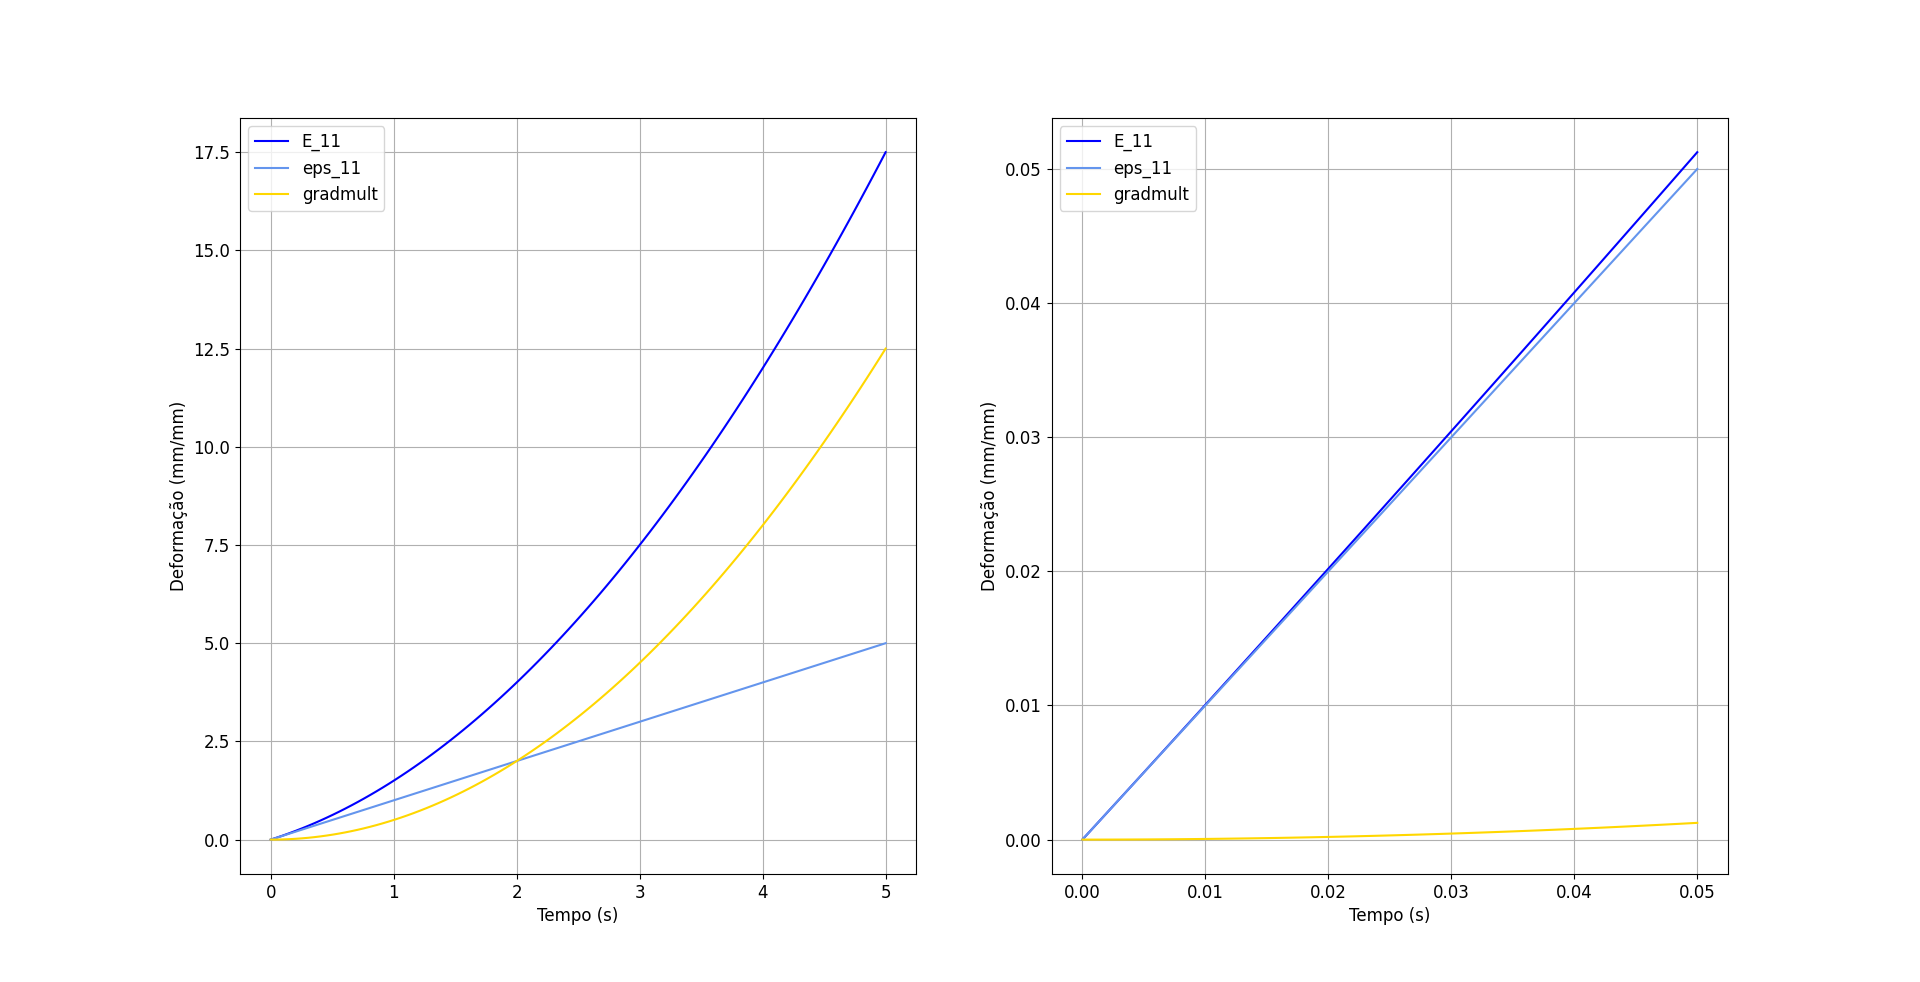
\includegraphics[width = \textwidth]{images/quest3ex.png}
	\label{fig:gradmult}
	\fonte{O autor (2020)}
\end{figure}

A figura \ref{fig:gradmult} denota a componente 11 das matrizes que representam o tensor de Green-Lagrange e o de deformações infinitesimais para um corpo submetido ao movimento supracitado. Observa-se que em baixos níveis de deformação, representados na imagem a direita, a parcela de maior ordem, chamada no gráfico de gradmult e correspondente à linha amarela, permanece com valor irrisório. Neste caso os valores do tensor de Green-Lagrange e o de deformações infinitesimais são semelhantes. Dado que computacionalmente o tensor infinitesimal tem custo menor ele é usado na grande maioria dos casos. De fato este é um tensor adequado para se trabalhar em casos onde há deformações e deslocamentos muito pequenos. A partir de certo ponto a parcela chamada de gradmult começa a ter influência significativa no tensor $ \gls{E} $ fazendo com que $ \gls{E} $ e $ \gls{eps} $ se distanciem. Por conta deste distanciamento o tensor infinitesimal é inadequado quando grandes deformações estão presentes. \par

Além dos tensores $ \gls{E} $ e $ \boldsymbol{\gls{eps}} $ existem outros que são muito usados para medir a deformação em um corpo contínuo, porém $\gls{E}$ é o mais relevante e os outros não serão abordados para manter a brevidade do trabalho.

\section{Princípios termomecânicos básicos}

\subsection{O balanço de massa}

A conservação de massa em sua forma global é apresentada na equação \ref{eq:consmassa}

\begin{equation}
    \int_{\Omega_r} \rho_r(\boldsymbol{X}) dV(\boldsymbol{X}) = \int_{\Omega} \rho(\boldsymbol{x},t) dv(\boldsymbol{x}) 
    \label{eq:consmassa}
\end{equation}

Onde $ \gls{Omegar} $ e $ \gls{Omega} $ são respectivamente a região ocupada pelo corpo na configuração material e espacial. Já $ \gls{rhor} $ e $ \gls{rho} $ são respectivamente a densidade do corpo na configuração material e espacial. Como o braço esquerdo da equação \ref{eq:consmassa} não depende do tempo, ao deriva-la o resultado é a equação \ref{eq:consmassa2}. O símbolo $ \dot{\overline{entidade}} $ significa a derivação no tempo da entidade em questão.
\begin{equation}
    \dot{\overline{\int_{\Omega} \rho(\boldsymbol{x,t}) dv(\boldsymbol{x})}} = 0
    \label{eq:consmassa2}
\end{equation}

O teorema do transporte de Reynold é aplicado na equação \ref{eq:consmassa2} tendo \ref{eq:consmassalocal0} como resultado. Admitindo que cada subdivisão do corpo deve respeitar a eq. \ref{eq:consmassalocal0} a forma local do balanço de massa, eq \ref{eq:consmassalocal}, é alcançada.\footnote{O teorema do transporte de Reynold pode ser encontrado em \cite{gurtin_fried_anand_2013} pg. 113}

\begin{align}
    \int_{\Omega} (\dot{\rho} + \rho div\boldsymbol{v})  dv &= 0 \label{eq:consmassalocal0} \\
    \dot{\rho} + \rho \; div\boldsymbol{v} &= 0 \label{eq:consmassalocal}
\end{align}

O balanço de massa deve ser respeitado tanto na formulação lagrangiana quanto na euleriana. Porém na formulação euleriana o balanço de massa se torna mais difícil de obedecer, já que pode haver fluxo do material através da malha. Este fluxo deve ser calculado e levado em consideração durante uma simulação. Quando se trata de uma descrição lagrangiana não há fluxo de material entre os elementos, sendo assim obedecer a conservação de massa se torna mais fácil, pois não há fluxo de massa entre elementos. 

\subsection{Balanço de momento linear e angular}

Um ponto importante para a discussão a seguir é assumir que o observador dos fenômenos está inerte. \par

Primeiro é definido um vetor $ \boldsymbol{r(x) = x - 0} $ que reside na configuração espacial, onde $ \boldsymbol{o} $ é a origem. São apresentados nas equações \ref{eq:linmoment} e \ref{eq:angmoment} o momento linear e angular respectivamente.

\begin{align}
    \boldsymbol{l}(\Omega) = \int_{\Omega} \rho \boldsymbol{v} dv \label{eq:linmoment} \\
    \boldsymbol{a}(\Omega) = \int_{\Omega} \boldsymbol{r} \times \rho \boldsymbol{v} dv \label{eq:angmoment}
\end{align}

Como uma consequência do balanço de massa, de acordo com \cite{gurtin_fried_anand_2013}, é possível escrever a derivada temporal do momento linear e angular da seguinte forma.

\begin{align}
   \dot{\overline{\boldsymbol{l}(\Omega)}} = \int_{\Omega} \rho \dot{\boldsymbol{v}} dv \label{eq:linmoment} \\
   \dot{\overline{\boldsymbol{a}(\Omega)}} = \int_{\Omega} \boldsymbol{r} \times \rho \dot{\boldsymbol{v}} dv \label{eq:angmoment}
\end{align}

Para completar o balanço falta discutir a aplicação de força no corpo. \cite{gurtin_fried_anand_2013} afirma que existem três tipos de força na mecânica do contínuo. 
\begin{itemize}
    \item Forças de contato entre regiões adjacentes que tem interseção ao longo de seu contorno.
    \item Forças de contato no contorno do corpo que são exercidas pelo ambiente.
    \item Forças de corpo em todos os pontos dele que são exercidas pelo ambiente.
\end{itemize}
De acordo com \cite{gurtin_fried_anand_2013} um dos maiores axiomas da mecânica do contínuo é a hipótese de Cauchy, que se refere às forças de contato e está representada graficamente na figura \ref{fig:hipotesecauchy}. 

\begin{figure}[H]
    \centering
    \caption{Representação gráfica da hipótese de Cauchy}
    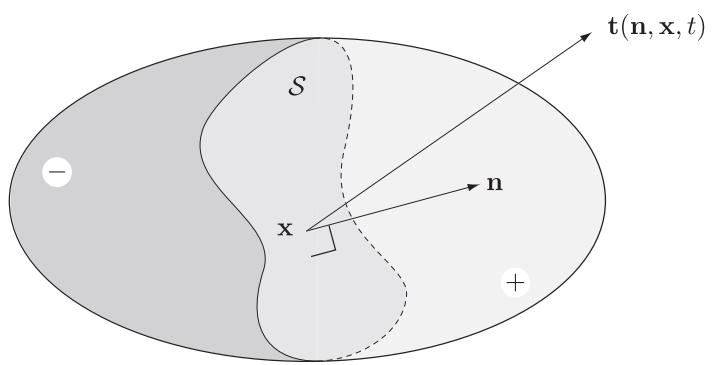
\includegraphics[width = 0.7 \textwidth]{images/hipoteseCauchy.png}
    \label{fig:hipotesecauchy}
    \fonte{\cite{gurtin_fried_anand_2013}}
\end{figure}

Em sua hipótese Cauchy insere um campo de tração superficial $ \boldsymbol{t}(\boldsymbol{x, n},t) $ definido para cada vetor unitário $ \boldsymbol{n} $, ponto $ \boldsymbol{x} $ pertencente ao corpo e tempo $ t $. O campo $ \boldsymbol{t}(\boldsymbol{x, n},t) $ tem a seguinte propriedade: Dada qualquer superfície espacial $ S $ pertencente ao corpo, $ \boldsymbol{t}(\boldsymbol{x, n},t) $ representa a força por unidade de área exercida através de $ S $. Esta força é aplicada no material na porção negativa e pelo material na porção positiva. \\

De acordo com \cite{gurtin_fried_anand_2013} para descobrir a força entre regiões adjacentes $ P $ e $D$ é necessário fazer uma integrar a tração ao longo da superfície $ S=P\cap D $. O resultado desta integração é a expressão \ref{eq:forçasup}.

\begin{equation}
    \int_{S} \boldsymbol{t(n)}\, da = \int_{S} \boldsymbol{t}(\boldsymbol{x, n},t) \, da(\boldsymbol{x})
    \label{eq:forçasup}
\end{equation}

A força total exercida pelo meio no corpo $ \Omega $ é descrita pela expressão \ref{eq:forçasuptot}. Onde $\boldsymbol{n}$ é a normal da superfície do corpo no ponto onde $\boldsymbol{t}$ está sendo avaliado e $\partial \Omega$ é toda a superfície do corpo.
\begin{equation}
    \int_{\partial \Omega} \boldsymbol{t(n)} \, da
    \label{eq:forçasuptot}
\end{equation}

O meio também pode exercer força ao longo de todo o volume do corpo. Um exemplo clássico é a força gravitacional. Esse tipo de força é descrita pela expressão \ref{eq:forçavoltot}.

\begin{equation}
    \int_{\Omega} \boldsymbol{b} \, dv
    \label{eq:forçavoltot}
\end{equation}

Conhecendo  $\gls{t}$ e $\gls{b}$ é possível definir a força e o momento líquidos em $ \gls{Omega}$, respectivamente expressões \ref{eq:forçaliq} e \ref{eq:momliq}.

\begin{align}
    \boldsymbol{f}(\Omega) = \int_{\partial \Omega} \boldsymbol{t(n)} \, da + \int_{\Omega} \boldsymbol{b} \, dv \label{eq:forçaliq} \\
    \boldsymbol{m}(\Omega) = \int_{\Omega} \boldsymbol{r} \times \boldsymbol{t(n)} \, da + \int_{\Omega} \boldsymbol{r} \times \boldsymbol{b} \, dv \label{eq:momliq}
\end{align}

A igualdade entre a derivada temporal do momento linear e a força total exercida no corpo expressa o balanço de momento linear, apresentado na expressão \ref{eq:linbal}. De maneira semelhante, a igualdade entre a derivada temporal do momento angular e o momento líquido exercido no corpo expressa o balanço de momento angular, apresentado na expressão \ref{eq:angbal}.

\begin{equation}
    \int_{\partial \Omega} \boldsymbol{t(n)} da + \int_{\Omega} \boldsymbol{b} dv = \int_{\Omega} \rho \dot{\boldsymbol{v}} dv \label{eq:linbal} 
\end{equation}

\begin{equation}
    \int_{\partial \Omega} \boldsymbol{r} \times \boldsymbol{t(n)} da + \int_{\Omega}    \boldsymbol{r} \times \boldsymbol{b} dv = \int_{\Omega} \boldsymbol{r} \times \rho \dot{\boldsymbol{v}} dv \label{eq:angbal} 
\end{equation}

O teorema de Cauchy é apresentado, sem prova-lo.\footnote{A prova do teorema de Cauchy pode ser encontrada em \cite{gurtin_fried_anand_2013} pg. 137} Uma consequência do balanço de momento linear é que existe um tensor $\gls{Cauchy}$ chamado tensor de tensões de Cauchy. Tal que a expressão \ref{eq:CauchyStress} é válida.

\begin{equation}
    \boldsymbol{t(n)} = \boldsymbol{\sigma n} \label{eq:CauchyStress}
\end{equation}

O teorema de Cauchy possibilita derivar a forma local tanto do balanço de momento linear quanto do balanço de momento angular. A derivação do balanço de momento linear local será feita a seguir, porém a mesma derivação para o balanço de momento angular local não será feita, por conta de sua extensão. Esta derivação pode ser encontrada em \cite{gurtin_fried_anand_2013} pg. 140 e resulta que $ \gls{Cauchy} = \gls{Cauchy}^T $, portanto o balanço de momento angular local implica a simetria do tensor de tensões de Cauchy. \par

Tendo como forma inicial o balanço de momento linear global, o teorema de Cauchy é aplicado chegando em \ref{eq:forma2}. Então ao aplicar o teorema do divergente ao primeiro termo do braço esquerdo a expressão \ref{eq:forma3} é obtida.\footnote{ O teorema do divergente implica na igualdade entre uma integral ao longo de um contorno e uma integral no volume deste contorno. Uma explicação deste pode ser encontrada em \cite{gurtin_fried_anand_2013} pg. 52. } A expressão \ref{eq:forma3} é válida para qualquer subdivisão do corpo, dado que qualquer uma delas tem as mesmas propriedades que o próprio corpo. A validade de \ref{eq:forma3} para qualquer subdivisão possibilita assumir que para qualquer ponto \ref{eq:locallinbal} deve ser atendida. O nome dado à expressão \ref{eq:locallinbal} é forma local espacial do balanço de momento linear. 
\begin{align}
    &\int_{\partial \Omega} \boldsymbol{t(n)} \, da + \int_{\Omega} \boldsymbol{b}\, dv = \int_{\Omega} \rho \dot{\boldsymbol{v}} \,dv \\
    &\int_{\partial \Omega} \boldsymbol{\sigma n} \,da + \int_{\Omega} \boldsymbol{b}\, dv = \int_{\Omega} \rho \dot{\boldsymbol{v}} \,dv \label{eq:forma2} \\ 
    &\int_{\Omega} \boldsymbol{div \sigma} \,dv + \int_{\Omega} \boldsymbol{b} \,dv = \int_{\Omega} \rho \dot{\boldsymbol{v}} \,dv  \label{eq:forma3} \\
    &div\gls{Cauchy} + \boldsymbol{b} = \rho \boldsymbol{\dot{v}} \label{eq:locallinbal}
\end{align}

\subsection{Balanço de potencias}

A equação \ref{eq:locallinbal}, o balanço local do momento linear, foi apresentada na configuração espacial. O balanço de potencias será trabalhado na configuração material e por conta disso é apresentada a equação \ref{eq:locallinbalmat}, que é o balanço de momento linear local na configuração material. Houve uma pequena alteração na notação usada até agora, na expressão \ref{eq:locallinbalmat} as quantidades relacionadas à configuração material não estão mais maiúsculas e sim com um $r$ subscrito. Além disso é inserido o primeiro tensor tensão de Piola-Kirchhoff $\gls{P}$, que pertence à configuração material. Ele é chamado de tensão de engenharia em uma curva tensão deformação de engenharia, enquanto o tensor tensão de Cauchy é a tensão real. 

\begin{equation} \label{eq:locallinbalmat}
    Div\gls{P} + \boldsymbol{b}_r = \rho_r \ddot{\mathcal{X}}
\end{equation}

É necessário apontar que $ div \boldsymbol{A} \neq Div \boldsymbol{A} $, dado que $ div \boldsymbol{A} = \frac{\partial A_{ij}}{\partial x_j} $ e $ Div \boldsymbol{A} = \frac{\partial A_{ij}}{\partial X_j} $, usando novamente a notação onde $ \boldsymbol{X = x_r}$. A transição do balanço de momento linear de local para global faz com que a equação \ref{eq:locallinbalmat} tenha a seguinte forma.

\begin{equation}
    \int_{\partial \Omega_r} \boldsymbol{Pn}\, da_r + \int_{\Omega_r} \boldsymbol{b}_r \,dv_r = \int_{\Omega} \rho_r \ddot{\mathcal{X}}\, dv_r
    \label{eq:globallinmat}
\end{equation}

O primeiro passo para chegar na expressão do balanço de potencias é fazer um produto interno à direita em \ref{eq:globallinmat} com a velocidade $ \dot{\mathcal{X}} $, gerando \ref{eq:globallinmat2}.

\begin{equation}
    \int_{\partial \Omega_r} \boldsymbol{Pn} \cdot \dot{\mathcal{X}} \, da_r + \int_{\Omega_r} \boldsymbol{b}_r \cdot \dot{\mathcal{X}} \,dv_r = \int_{\Omega} \rho_r  \ddot{\mathcal{X}} \cdot \dot{\mathcal{X}} \,dv_r
    \label{eq:globallinmat2}
\end{equation}

O braço direito da equação acima é equivalente à taxa de variação da energia cinética, de acordo com \ref{eq:cineneqv}.\footnote{Basta derivar o braço direito usando a regra da multiplicação para chegar no braço esquerdo.}

\begin{equation} \label{eq:cineneqv}
    \int_{\Omega} \rho_r  \ddot{\mathcal{X}} \cdot \dot{\mathcal{X}} dv_r = \frac{d}{dt} \int_{\Omega_r} \frac{1}{2}\rho_r |\dot{\mathcal{X}}|^2 dv_r= \dot{\overline{\mathcal{K}(\Omega_r)}}
\end{equation}

O foco agora é o primeiro termo do braço direito da equação \ref{eq:globallinmat2}. Ao aplicar o teorema do divergente a este termo a seguinte expressão é atingida.\footnote{Tal identidade é apresentada na pg. 56 de \cite{gurtin_fried_anand_2013}}

\begin{equation}
    \int_{\partial \Omega_r} \boldsymbol{Pn} \cdot \dot{\mathcal{X}} \,da_r = \int_{\Omega} (\dot{\mathcal{X}} \cdot Div\boldsymbol{P} + \boldsymbol{P} : \dot{\boldsymbol{F}} )\,dv_r
    \label{eq:transpowerbalance}
\end{equation}

Perceba que no primeiro termo dentro da integral no braço direito de  \ref{eq:transpowerbalance} é possível aplicar o balanço de momento linear da forma local, $ Div \boldsymbol{P} = \rho_r \ddot{\mathcal{X}} - \boldsymbol{b}_r $, obtendo o balanço de potências na configuração material. 

\begin{equation} \label{eq:baldepotencias}
     \underbrace{\int_{\partial \Omega_r} \gls{P}\boldsymbol{n}_r \cdot \dot{\mathcal{X}} \,da_r + \int_{\Omega_r} \boldsymbol{b}_r \cdot \dot{\mathcal{X}} \,dv_r}_\text{Potência externa $\gls{convpower}$ } = \underbrace{\int_{\Omega_r} \boldsymbol{P}: \dot{\boldsymbol{F}} \,dv_r}_\text{Potência interna $\gls{Pint}$ } + \underbrace{\frac{d}{dt} \int_{\Omega_r} \frac{1}{2}\rho_r |\dot{\mathcal{X}}|^2 \,dv_r}_\text{Variação da energia cinética $\dot{\mathcal{K}}_(\Omega_r)$} 
\end{equation}

\subsection{Balanço de energia}

O balanço de energia ou a primeira lei da termodinâmica quando aplicado ao contínuo toma, em sua forma global, a forma apresentada na expressão \ref{eq:primeiralei}. Nele o termo $ \gls{e_r} $ denota a energia interna do corpo na configuração material. O vetor $\boldsymbol{q}_r$ é o fluxo de calor para o corpo e $q_r$ é um escalar que representa fluxos de calor irradiados.

\begin{align}  \label{eq:primeiralei}
  \int_{\Omega_r} (\dot{e_r} + \frac{1}{2} \rho_r|\ddot{\mathcal{X}}|^2) dv_r = -&\int_{\partial \Omega_r} \boldsymbol{q}_r \cdot \boldsymbol{n}_r da_r + \int_{\Omega} q_r dv_r + \\ \notag 
    &\int_{\partial \Omega_r} \boldsymbol{Pn_r} \cdot \dot{\mathcal{X}} da_r + \int_{\Omega} \boldsymbol{b}_r \cdot \dot{\mathcal{X}} dv_r
\end{align}

Usando o balanço de potencias \ref{eq:baldepotencias} chega-se na forma do balanço de energia mais utilizada em códigos de propagação de ondas.\footnote{Este é um nome alternativo ao jargão que vem do inglês Hydrocode.} Nesta forma $\dot{\gls{Etot}}$ é a derivada no tempo da energia total do corpo.

\begin{equation} \label{eq:balenergia}
    \underbrace{\int_{\Omega_r} \dot{e_r} dv_r}_\text{$\dot{\mathcal{E}}_{tot}(\Omega_r)$} = \underbrace{\int_{\partial \Omega_r} \gls{P}\boldsymbol{n}_r \cdot \dot{\mathcal{X}} da_r + \int_{\Omega_r} \boldsymbol{b}_r \cdot \dot{\mathcal{X}} dv_r}_\text{$\gls{convpower}$ } \underbrace{-\int_{\partial \Omega_r} \boldsymbol{q}_r \cdot \boldsymbol{n}_r da_r + \int_{\Omega} q_r dv_r}_\text{Fluxo de calor $ \gls{Q} $}
\end{equation}

A equação \ref{eq:balenergia} termina a descrição dos princípios termo-mecânicos básicos. A segunda lei da termodinâmica não foi citada por ter maior representação como uma limitação à teoria constitutiva dos materiais, elas é usada para cunhar modelos consistentes. A teoria constitutiva não será abordada em termos de suas das limitações e teorias energéticas envolvidas, no entanto os modelos constitutivos serão apresentados e discutidos de forma expositiva.




